%%%%%%%%%%%%%%%%%%%%%%%%%%%%%%%%%%%%%%%%%%%%%%%%%%%%%%%%%%%%%%%%%%%%%%%%%%%%%%%%%%
\begin{frame}[fragile]\frametitle{}
\begin{center}
{\Large Career in AI: Tools}
\end{center}
\end{frame}


%%%%%%%%%%%%%%%%%%%%%%%%%%%%%%%%%%%%%%%%%%%%%%%%%%%%%%%%%%%%%%%%%%%%%%%%%%%%%%%%%%
\begin{frame}[fragile]\frametitle{Scikit-Learn}
\begin{columns}[T]
\begin{column}{.48\textwidth}

\includegraphics[width=\linewidth]{sklearn.png}
\end{column}
\begin{column}{.48\textwidth}
\begin{itemize}
\item Popular machine learning library
\item Provides simple and efficient tools for data mining and data analysis
\end{itemize}
\end{column}
\end{columns}
\end{frame}

%%%%%%%%%%%%%%%%%%%%%%%%%%%%%%%%%%%%%%%%%%%%%%%%%%%%%%%%%%%%%%%%%%%%%%%%%%%%%%%%%%
\begin{frame}[fragile]\frametitle{TensorFlow}
\begin{columns}[T]
\begin{column}{.48\textwidth}

\includegraphics[width=\linewidth]{TensorFlow_logo.svg.png}
\end{column}
\begin{column}{.48\textwidth}
\begin{itemize}
\item TensorFlow is an open-source library for machine learning and artificial intelligence
\item Developed by the Google Brain team
\item Allows easy deployment of computation to CPUs, GPUs, and TPUs
\item Provides a Python API as well as APIs for other languages
\end{itemize}
\end{column}
\end{columns}
\end{frame}

%%%%%%%%%%%%%%%%%%%%%%%%%%%%%%%%%%%%%%%%%%%%%%%%%%%%%%%%%%%%%%%%%%%%%%%%%%%%%%%%%%
\begin{frame}[fragile]\frametitle{Key Features}
\begin{itemize}
\item Eager Execution for interactive coding
\item Keras for building and training models
\item TensorFlow Hub for reusable models
\item TensorFlow Lite for mobile and embedded devices
\item TensorFlow Extended (TFX) for model pipelines
\end{itemize}
\end{frame}

%%%%%%%%%%%%%%%%%%%%%%%%%%%%%%%%%%%%%%%%%%%%%%%%%%%%%%%%%%%%%%%%%%%%%%%%%%%%%%%%%%
\begin{frame}[fragile]\frametitle{Code Example: MNIST Digits Classification}
\begin{verbatim}
import tensorflow as tf

mnist = tf.keras.datasets.mnist
(x_train, y_train), (x_test, y_test) = mnist.load_data()

model = tf.keras.models.Sequential([
  tf.keras.layers.Flatten(input_shape=(28, 28)),
  tf.keras.layers.Dense(128, activation='relu'),
  tf.keras.layers.Dropout(0.2),
  tf.keras.layers.Dense(10, activation='softmax')
])

model.compile(optimizer='adam', loss='sparse_categorical_crossentropy', metrics=['accuracy'])
model.fit(x_train, y_train, epochs=5)
model.evaluate(x_test, y_test)
\end{verbatim}
\end{frame}

%%%%%%%%%%%%%%%%%%%%%%%%%%%%%%%%%%%%%%%%%%%%%%%%%%%%%%%%%%%%%%%%%%%%%%%%%%%%%%%%%%
\begin{frame}[fragile]\frametitle{Future Developments}
\begin{itemize}
\item Improved support for multi-cloud and hybrid environments
\item Continued focus on performance, scalability, and efficiency
\item Integration with emerging hardware like AI accelerators
\item Expanded model libraries and pre-trained models
\item Advanced features for research and experimentation
\end{itemize}
\end{frame}

%%%%%%%%%%%%%%%%%%%%%%%%%%%%%%%%%%%%%%%%%%%%%%%%%%%%%%%%%%%%%%%%%%%%%%%%%%%%%%%%%%
\begin{frame}[fragile]\frametitle{Pytorch}
\begin{columns}[T]
\begin{column}{.48\textwidth}

\includegraphics[width=\linewidth]{2560px-PyTorch_logo_black.svg.png}
\end{column}
\begin{column}{.48\textwidth}
\begin{itemize}
\item Open-source machine learning library
\item Developed by Facebook's AI Research lab (FAIR)
\end{itemize}
\end{column}
\end{columns}
\end{frame}

%%%%%%%%%%%%%%%%%%%%%%%%%%%%%%%%%%%%%%%%%%%%%%%%%%%%%%%%%%%
\begin{frame}[fragile]\frametitle{ChatGPT - A Tipping Point for Generative AI}
    \begin{itemize}
        \item Released by OpenAI in November 2022
        \item Generative AI chatbot
        \item Rapid worldwide popularity
        \item 1 million users in 5 days
        \item Netflix took 3.5 years for same user count
        \item 100 million monthly active users by January 2023
        \item Fastest-growing application in history
    \end{itemize}
\end{frame}

%%%%%%%%%%%%%%%%%%%%%%%%%%%%%%%%%%%%%%%%%%%%%%%%%%%%%%%%%%%
\begin{frame}[fragile]\frametitle{Midjourney: Image Generation Model}
    
    \begin{itemize}
        \item Developed by Midjourney Inc.
        \item Released in July 2022
        \item Architecture details undisclosed
        \item High-quality image generation
        \item Wide variety of styles and genres
    \end{itemize}
	
\end{frame}

%%%%%%%%%%%%%%%%%%%%%%%%%%%%%%%%%%%%%%%%%%%%%%%%%%%%%%%%%%%
\begin{frame}[fragile]\frametitle{LLaMA}

    \begin{itemize}
        \item February 2023: Meta releases LLM "LLaMA"
        \item LLaMA: 65-billion parameter model
        \item Trained on extensive text and code dataset
    \end{itemize}
	
Significance of LLaMA Release

    \begin{itemize}
        \item One of the largest public LLMs
        \item Suited for complex and challenging tasks
        \item Open source, initially for research purposes
        \item Model weights leaked online, accessible to all
        \item Sparked development of numerous open source LLMs
    \end{itemize}
\end{frame}


%%%%%%%%%%%%%%%%%%%%%%%%%%%%%%%%%%%%%%%%%%%%%%%%%%%%%%%%%%%
\begin{frame}[fragile]\frametitle{Anthropic Claude}


\begin{columns}
    \begin{column}[T]{0.6\linewidth}
		\begin{center}
		\includegraphics[width=\linewidth,keepaspectratio]{promptengg90}

		{\tiny (Ref: The Complete Prompt Engineering for AI Bootcamp (2023))}
		\end{center}	
    \end{column}
    \begin{column}[T]{0.4\linewidth}
		Created by Anthropic 
		https://console.anthropic.com/ or API
		Uses Constitutional AI rather than RLHF
		
		Constitutional AI trains to follow a set of high-level principles or rules, such as a constitution, that specify the desired behavior and outcomes of the system.
		RLHF uses human feedback, such as ratings, preferences, or corrections, to optimize a language model or an agent’s policy using reinforcement learning
    \end{column}
  \end{columns}
\end{frame}

%%%%%%%%%%%%%%%%%%%%%%%%%%%%%%%%%%%%%%%%%%%%%%%%%%%%%%%%%%%
\begin{frame}[fragile]\frametitle{Github Copilot: Breakthrough Coding Assistant}
    
    \begin{itemize}
        \item OpenAI introduced Github Copilot in 2021
        \item Built on GPT-3 architecture
        \item Fine-tuned on millions of public code lines
        \item Auto-completes and suggests code
        \item Supports multiple programming languages
    \end{itemize}
\end{frame}

%%%%%%%%%%%%%%%%%%%%%%%%%%%%%%%%%%%%%%%%%%%%%%%%%%%%%%%%%%%
\begin{frame}[fragile]\frametitle{Low/No Code Platform : Knime}
\begin{columns}[T]
\begin{column}{.48\textwidth}

\includegraphics[width=\linewidth]{knime-og-knime-logo.jpg}
\end{column}
\begin{column}{.48\textwidth}
\begin{itemize}
\item Open-source low/no code platform for data analytics, reporting, and integration
\item Offers visual programming interface
\end{itemize}
\end{column}
\end{columns}
\end{frame}

%%%%%%%%%%%%%%%%%%%%%%%%%%%%%%%%%%%%%%%%%%%%%%%%%%%%%%%%%%%
\begin{frame}[fragile]\frametitle{Low/No Code Platforms: Weka}
\begin{columns}[T]
\begin{column}{.48\textwidth}

\includegraphics[width=\linewidth]{weka-logo.jpg}
\end{column}
\begin{column}{.48\textwidth}
\begin{itemize}
\item Open-source low/no code platform for data mining and machine learning
\item Provides tools for data preprocessing, classification, regression, clustering, and association rules
\end{itemize}
\end{column}
\end{columns}
\end{frame}

%%%%%%%%%%%%%%%%%%%%%%%%%%%%%%%%%%%%%%%%%%%%%%%%%%%%%%%%%%%
\begin{frame}[fragile]\frametitle{Cloud Platforms: GCP}
\begin{columns}[T]
\begin{column}{.48\textwidth}
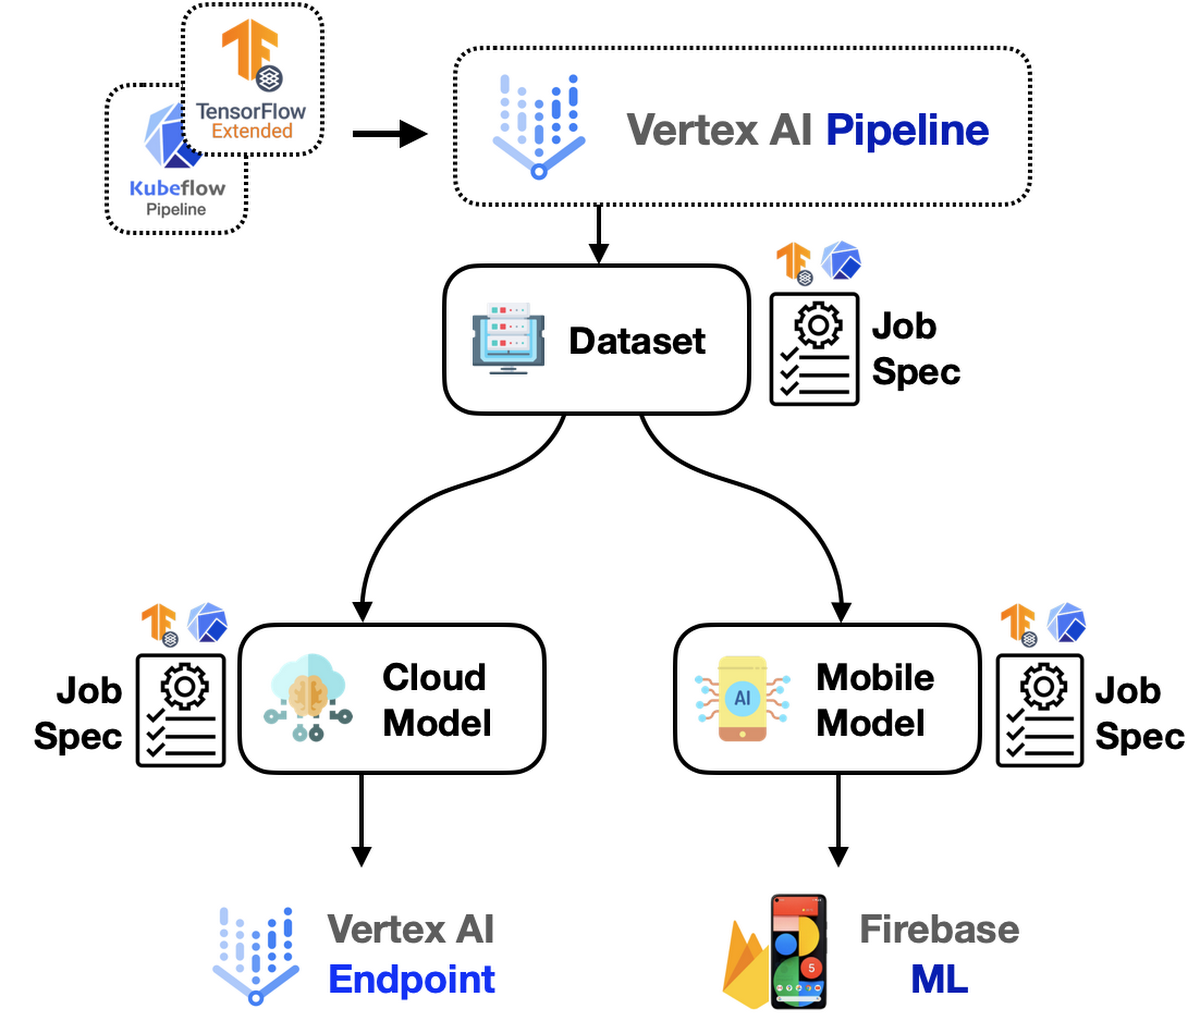
\includegraphics[width=\linewidth]{gcp_vertex_ai.png}
\end{column}
\begin{column}{.48\textwidth}
\begin{itemize}
\item Google Cloud Platform (GCP)
\item Cloud computing services by Google
\item Offers various AI and machine learning services such as Gen AI Studio, Vertex AI, etc.
\end{itemize}
\end{column}
\end{columns}
\end{frame}

%%%%%%%%%%%%%%%%%%%%%%%%%%%%%%%%%%%%%%%%%%%%%%%%%%%%%%%%%%%
\begin{frame}[fragile]\frametitle{Cloud Platforms; Azure}
\begin{columns}[T]
\begin{column}{.48\textwidth}
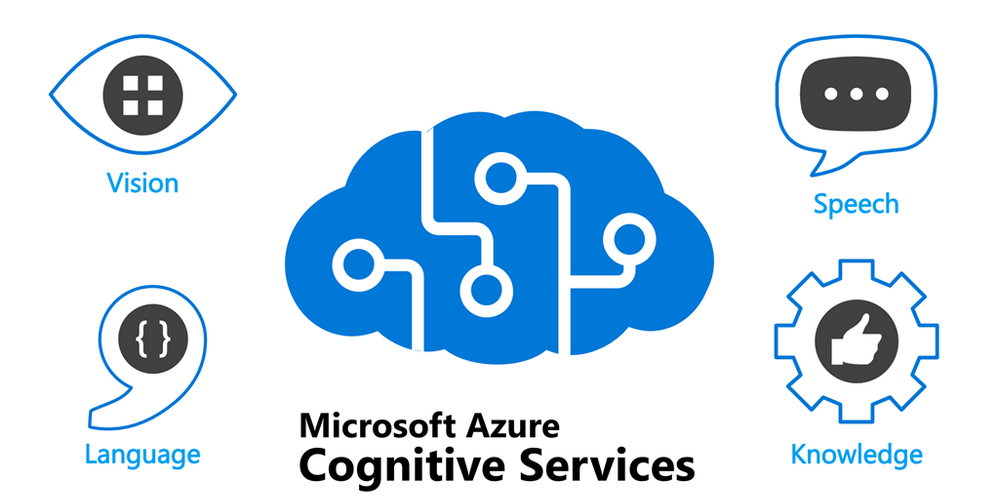
\includegraphics[width=\linewidth]{azure-cognitive-services.png}
\end{column}
\begin{column}{.48\textwidth}
\begin{itemize}
\item Microsoft Azure
\item Cloud computing services by Microsoft
\item Provides AI and machine learning services like Azure Machine Learning, Cognitive Services, etc.
\end{itemize}
\end{column}
\end{columns}
\end{frame}

%%%%%%%%%%%%%%%%%%%%%%%%%%%%%%%%%%%%%%%%%%%%%%%%%%%%%%%%%%%
\begin{frame}[fragile]\frametitle{Cloud Platforms: AWS}
\begin{columns}[T]
\begin{column}{.48\textwidth}

\includegraphics[width=\linewidth]{aws_logo}
\end{column}
\begin{column}{.48\textwidth}
\begin{itemize}
\item Amazon Web Services (AWS)
\item Cloud computing services by Amazon
\item Offers AI and machine learning services such as Amazon SageMaker, Amazon Comprehend, etc.
\end{itemize}
\end{column}
\end{columns}
\end{frame}
